\documentclass[a4paper]{ltjsarticle}
\usepackage{tikz}
\usepackage{listings}
\usepackage{xcolor}

\lstset{
  basicstyle=\ttfamily\small,        % フォントとサイズ
  keywordstyle=\color{blue},         % キーワードの色
  commentstyle=\color{gray},         % コメントの色
  stringstyle=\color{red},           % 文字列リテラルの色
  numberstyle=\tiny\color{gray},     % 行番号のスタイル
  numbers=left,                      % 行番号を左に表示
  stepnumber=1,                      % 行番号の間隔
  frame=single,                      % 枠で囲む
  breaklines=true,                   % 長い行を折り返す
  language=C                         % デフォルト言語
}

\begin{document}

\begin{center}
{\LARGE 計算数学特論 第1回レポート}\\[1em]
学籍番号:\underline{62216580}\\
氏名:\underline{平田智也}\\
提出日:\underline{2025/06/08}
\end{center}

選択した問題: 2, 5. 根拠には自作のC言語の
プログラムを用いていて, 二つとも同じプログラムの中で,
main関数を分ける形で分割して記述した.

問題2

(a)この問題は二部グラフが完全マッチングを持つか判定する問題として定式化できることを示せ.

頂点集合を各マス目として, 隣接している⇔辺を結ぶ, としてできるグラフを考える.
このグラフは連結であることを仮定してよい. ( なぜならば, 非連結であった場合には, それぞれの連結成分が
タイリングできるかを帰納的に調べることになるだけで, 連結成分が複数存在する場合は無視してよいからである.)

また, すべてのタイルは正方形であって, すべてが整然とならんでいることから,
すべてのタイルを2次元平面における格子点に倣って名づけることができる.

今回は, 適宜そのタイルを大きく拡張して一つの大きな長方形にしたときに,
一番左下になるマスに(0, 0)と名づけ, 以下右に1つ進むたびに
第1成分に1を足し, 上に1つ進むたびに第2成分に1を足してそのマス目の名前
とする.

\begin{center}
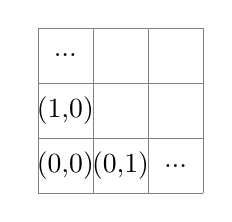
\begin{tikzpicture}[scale=0.7]
  % 5x5のマス目
  \draw[step=1cm,gray,very thin] (0,0) grid (3,3);

  % 各マスの中央に文字を配置
  \node at (0.5,0.5) {(0,0)};
  \node at (0.5,1.5) {(1,0)};
  \node at (1.5,0.5) {(0,1)};
	\node at (2.5,0.5) {...};
	\node at (0.5,2.5) {...};
\end{tikzpicture}
\end{center}

以下は問題の図であるが, これに名前を付けた上で, 以下に示すように, 第1成分と第2成分の和が
奇数の場合は赤く, 偶数の場合は青く塗っていく.(書いていない, 塗られていないところは適宜
例に従って補完されるものとする.)

\begin{center}
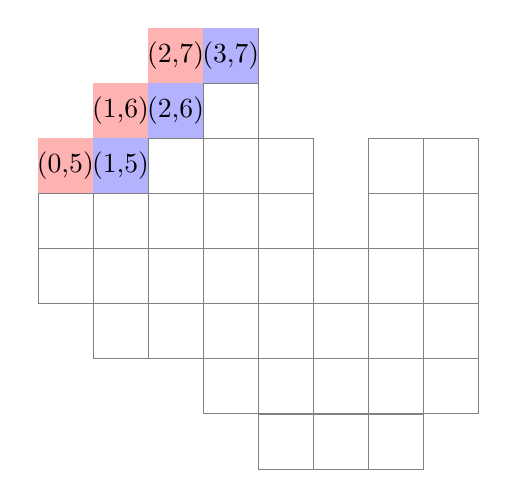
\begin{tikzpicture}[scale=0.7]
	\draw[step=1cm,gray,very thin] (0,3) grid (5,6);
	\draw[step=1cm,gray,very thin] (1,2) grid (8,4);
	\draw[step=1cm,gray,very thin] (6,4) grid (8,6);
	\draw[step=1cm,gray,very thin] (3,1) grid (8,2);
	\draw[step=1cm,gray,very thin] (4,0) grid (7,1);
	\draw[step=1cm,gray,very thin] (1,6) grid (2,7);
	\draw[step=1cm,gray,very thin] (2,6) grid (4,8);

	\fill[blue!30] (3,7) rectangle (4,8);
	\fill[blue!30] (2,6) rectangle (3,7);
	\fill[blue!30] (1,5) rectangle (2,6);

	\fill[red!30] (2,7) rectangle (3,8);
	\fill[red!30] (1,6) rectangle (2,7);
	\fill[red!30] (0,5) rectangle (1,6);
	\node at (3.5, 7.5) {(3,7)};
	\node at (2.5, 7.5) {(2,7)};
	\node at (2.5, 6.5) {(2,6)};
	\node at (1.5, 6.5) {(1,6)};
	\node at (1.5, 5.5) {(1,5)};
	\node at (0.5, 5.5) {(0,5)};
\end{tikzpicture}
\end{center}

こうして色を塗っていくと, ドミノはちょうど赤いマスと青いマスを
一つずつ覆うようにしか配置できないことが分かる.
言い換えれば, どの隣接する赤いマスと青いマスが一つのタイルに
よって覆われるか, ということと同じことである.

従って, これは赤く塗られたマスを頂点集合A, 青く塗られたマスを
頂点集合Bとしたときに, A, B間に完全マッチングが存在するかどうか,
という問題に帰着できることが分かる.

(b)上の図のチェックボードはドミノでタイリングできるだろうか.

不可能である. 授業で紹介されたKuhn's Algorithmを今回の
グラフに適用し, 最大マッチング数が20(\neq 21=|A|=|B|)であることより示す.
以下は, 提出ファイルを適宜参照されたい.必要がある場合, 参照元を示しながら記述する.

a2.txtには, A, B間の隣接行列が格納されている.頂点番号は,
あらためて, 左上から, 以下のように, 0, 1, 2, ..., 20とついている.

\begin{center}
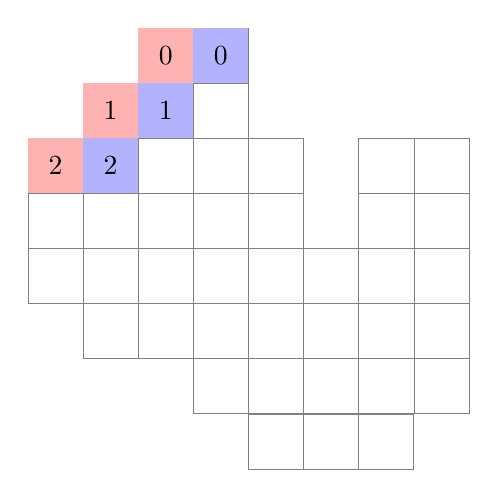
\begin{tikzpicture}[scale=0.7]
	\draw[step=1cm,gray,very thin] (0,3) grid (5,6);
	\draw[step=1cm,gray,very thin] (1,2) grid (8,4);
	\draw[step=1cm,gray,very thin] (6,4) grid (8,6);
	\draw[step=1cm,gray,very thin] (3,1) grid (8,2);
	\draw[step=1cm,gray,very thin] (4,0) grid (7,1);
	\draw[step=1cm,gray,very thin] (1,6) grid (2,7);
	\draw[step=1cm,gray,very thin] (2,6) grid (4,8);

	\fill[blue!30] (3,7) rectangle (4,8);
	\fill[blue!30] (2,6) rectangle (3,7);
	\fill[blue!30] (1,5) rectangle (2,6);

	\fill[red!30] (2,7) rectangle (3,8);
	\fill[red!30] (1,6) rectangle (2,7);
	\fill[red!30] (0,5) rectangle (1,6);
	\node at (3.5, 7.5) {0};
	\node at (2.5, 7.5) {0};
	\node at (2.5, 6.5) {1};
	\node at (1.5, 6.5) {1};
	\node at (1.5, 5.5) {2};
	\node at (0.5, 5.5) {2};
\end{tikzpicture}
\end{center}

README.mdに記載した通りにコンパイルし, 実行ファイル./report2を実行すると, 「20」が出力される.
必要があれば, Bの中の頂点が対応しているAの頂点を示す配列match\_toを表示する
(print\_array\_int(match\_to, b);で表示可能)ことで, -1の未接続の頂点が
処理されることなく処理が終わっていることが確認できる.

よって, この二部グラフの最大マッチング数は20であり, 完全マッチングは存在しない.
したがって, タイリングはできない.

問題5

最小コスト完全マッチングを求めるアルゴリズムを実装し, 実験せよ.

上記と同じく, 実行ファイル./report5を実行すると, b1.txtからb5.txt
に対してHungarian's Algorithmを適用し, それぞれの
頂点数$|A|$, $|B|$, 辺の数mと, 実行時間, 最小コストが出力される.
また, 参考までに理論計算量である$n^2 * m$の具体的な値も出力した.

\begin{table}[htbp]
\centering
\caption{Hungarianアルゴリズムの実行結果まとめ}
\begin{tabular}{|c|c|c|c|c|c|}
\hline
ファイル名 & $|A|$ & $|B|$ & $n^2 \times m$ & 実行時間 [秒] & 最小コスト \\
\hline
b1.txt & 50  & 109  & 68,890,725   & 0.004 & 0.571276 \\
b2.txt & 255 & 189  & 455,418,896  & 0.059 & 1.740562 \\
b3.txt & 25  & 30   & 1,134,375    & 0.001 & 1.065767 \\
b4.txt & 430 & 381  & 2,337,608,163 & 0.193 & 1.602832 \\
b5.txt & 23  & 400  & 823,073,400  & 0.006 & 0.085391 \\
\hline
\end{tabular}
\end{table}

\newpage

\begin{lstlisting}[language=C]
double hungarian(double **cost, int a, int b, int *match_to) {
    Hungarian_ctx ctx;
    int n, i, i0, j, j0, j1;
    double result, delta, cur;
    n = (a > b) ? a : b;
    if (!init_hungarian_ctx(&ctx, n))
        return (-1);
    result = 0.0;			// ①
    for (i = 1; i <= a; i++) {
        ctx.p[0] = i;
        init_row(&ctx);
        j0 = 0;
        ctx.way[j0] = 0;		// ②
        do {
            ctx.used[j0] = 1;
            i0 = ctx.p[j0];
            j1 = 0;
            for (j = 1; j <= b; j++) {
                if (!ctx.used[j]) {	// ③
                    cur = cost[i0 - 1][j - 1] - ctx.u[i0] - ctx.v[j];
                    if (cur < ctx.minv[j]) {
                        ctx.minv[j] = cur;
                        ctx.way[j] = j0;
                    }
                }
            }
            find_min(&ctx, &delta, &j1); // ④
            update_labels(&ctx, delta); // ⑤
            j0 = j1;
        } while (ctx.p[j0] != 0); 	// ⑥
        augment_path(&ctx, j0); 	// ⑦
    }
    for (j = 1; j <= b; j++) {		// ⑧
        if (ctx.p[j] > 0 && ctx.p[j] <= a)
            match_to[j - 1] = ctx.p[j] - 1;
        else
            match_to[j - 1] = -1;
    }
    for (j = 1; j <= b; j++) {
        if (match_to[j - 1] != -1)
            result += cost[match_to[j - 1]][j - 1];
    }
    free_hungarian_ctx(&ctx);
    return result;
}
\end{lstlisting}

すべてのソースコードは長いため, 最も重要な関数のみを掲載する.詳細は別途提出した
ソースコードを参照されたい.

Hungarian\_ctxは以下のようになっている.

\begin{lstlisting}[language=C]
typedef struct 	Hungarian_ctx
{
	int 	n;	// a, bのうち大きい方
	double 	*u;	// 双対変数を格納する配列
	double 	*v;	// 双対変数を格納する配列
	int 	*p;	// 現在のマッチングの対応を記録する配列
	int 	*way;	// 増加パスを辿るための補助配列
	double 	*minv;	// 割り当て可能な最小コストを一時的に保持する配列
	int 	*used;	// 探索済みかどうかを保持する配列
}				Hungarian_ctx;
\end{lstlisting}

・処理の流れの簡単な説明

①ここまでが初期化

②Aの頂点一つずつにつき, コスト最小の頂点を探す.

③相補性条件をチェックする.

④minvから最小の頂点を探し, 次に辿る頂点j1を記録する.

⑤双対変数を更新する.

⑥p[j0]が0 ⇔ 割り当てられなかったということなので, ループを抜ける.

⑦j0からway配列を辿り, 配列pを更新する.

⑧最終結果を記録する.

・頂点数, 辺数が増えることによる処理時間への影響

表1を見ると, 概ね理論計算量にともなって実行時間が増加する傾向にあるが,
一方でb5.txtに見られるように, 頂点数に偏りがある二部グラフの場合は
理論上の計算量よりも小さい計算量で終了していることが分かる.

・nが大きくなった際の最適値の変化

表1を見ると, b2.txtにおける最適値は約1.74であるのに対し,
頂点数, 辺の数ともに増加しているb4.txtにおいて, 約1.60と,
むしろ最適値は減少していることは注目すべきである.もちろん,
これは乱数生成を使っているので, 偶然に小さい値が何個も登場した, という
ことは考えられるが, この結果から, 少なくとも「\infty に発散する」
という結論は出しにくい.むしろ, 1.7前後に収束する可能性も示唆される.

このアルゴリズムにおける最適値は, 対応するマッチングのコストの合計である.すなわち,
\[
m = \min\{|A|, |B|\}
\]
の個数分のコストの合計であるが,
この一つ一つが平均して $\alpha / m$ であると言えれば, 最適値は収束すると考えられる.

独立な一様分布であることを仮定すると,
個数が増えるにつれて最小値の期待値も減少していくと考えられるため, それが収束するかどうかは
一考の余地がある.ただし, この挙動はコストの確率分布に大きく依存すると考えられる.

\end{document}
